%%%%%%%%%%%%%%%%%%%%%%%%%
% Dokumentinformationen %
%%%%%%%%%%%%%%%%%%%%%%%%%
\newcommand{\titleinfo}{Leistungselektronik - Formelsammlung}
\newcommand{\authorname}{\href{mailto:lmazzole@hsr.ch}{L. Mazzoleni}}
%\RequirePackage{luatex85}
%\def\pgfsysdriver{pgfsys-pdftex.def}
\newcommand{\authoremail}{\href{mailto:lmazzole@hsr.ch}{lmazzole@hsr.ch}}
\newcommand{\versioninfo}{$ Entwurf $}

\include{header/header}
\usepackage{nicefrac}
\usepackage{tikz}


%%%%%%%%%%%%%%%%%%%%%%%%%%%%%%%%%%%%%%%%%%%%%%%%%%%%%%%%%%%%%%%%%%%%%%%%%%%%%%%%%%%%%%%%%%%%%%%%

\begin{document}  
\maketitle
\vspace{-2.5cm}
\setcounter{tocdepth}{2}
\tableofcontents
\thispagestyle{empty}
\clearpage
\input{sections/V1}
\section{Diode}
Eine Diode besteht aus PN übergängen und ist deswegen ein nichtlineares Element:
\begin{multicols}{2}
     \begin{minipage}{\linewidth}
         \begin{tabular}{ll}
             $ U_{DBR} $    & Durchbruchspanung  \\ 
             $ U_D $        & Diffusionsspannung (0.7V Si)  \\ 
             $ U_F $        & Flussspannung \\ 
             $ U_R $        & Sperrspannung  \\ 
              $ i_F $       & Diffusionsstrom, Strom in Durchlassrichtung  \\ 
              $ i_R $       & Leckstrom, Strom in Sperrichtung \\ 
            \end{tabular} 
        \end{minipage}
        
         \includegraphics[width=0.8\linewidth]{images/kennlinieDiode}
\end{multicols}
\vspace{-1.5cm}
\begin{multicols}{2}
     \begin{minipage}{\linewidth}
         \begin{tabular}{ll}
             $ i_f ,\; u_F $& Durchlassrichtung\\
             $ U_{T0} $& Schwellenspannung\\
             $ r_f= \dfrac{\diff U_F}{\diff i_F} $& Differenzieller Durchlasswiderstand\\
            \end{tabular}       
    \end{minipage}
        
        \includegraphics[width=0.4\linewidth]{images/dDiodeKennlinie}
\end{multicols}
\vspace{-1.5cm}
\subsection{Ersatzschaltbild}
\begin{multicols}{4}
    \begin{minipage}{\linewidth}
        \textbf{Reale Diode} \raggedright \newline\newline
        \includegraphics[width=0.7\linewidth]{images/realeDiode}
    \end{minipage}
    
    \begin{minipage}{\linewidth}
        \textbf{Ideale Diode ($ D_1 $)} \raggedright \newline\newline
        \includegraphics[width=0.7\linewidth]{images/idealeDiode}
    \end{minipage}
    
    \begin{minipage}{\linewidth}
        \textbf{Diode $ D_1 $ mit der Schwellenspannung $  D_2 $} \raggedright
        \includegraphics[width=0.6\linewidth]{images/idealeDiodeSP}
    \end{minipage}
    
    \begin{minipage}{\linewidth}
        \textbf{Diode $ D_2 $ mit dem Durchlasswiderstand($ D_3 $)} \raggedright
        \includegraphics[width=0.6\linewidth]{images/idealeDiodeSPR}    
    \end{minipage}                       
\end{multicols}
\begin{multicols}{2}
\subsection{Grundformeln}
\begin{tabular}{ll}
    \textbf{Flussspannung}&\[ u_F = U_{T0} + i_F \cdot r_F \]\\
    \textbf{Momentanleistung}&\[ p(t)=u_F(t)\cdot i_F(t) \]\\
    \textbf{Verlustleistung}&\[ P_v=U_{TO}\cdot I_{FAV}+r_F\cdot I_{FRMS}^2 \]\\
    $ I_{FAV}$ & arithmetische Mittelwert von $ i_F $\\
    $ I_{FRMS} $ & Effektivwert von $ i_F $\\    
\end{tabular}

\hspace{0.5cm}\includegraphics[width=0.6\linewidth]{images/ESBDiode} 
\end{multicols}

\subsection{Schaltverhalten und Schaltverluste}
    \begin{minipage}{0.7\linewidth}
        \raggedright
        \textbf{Durchlassverzug:}\newline
        freie Ladungsträger müssen zuerst die Ladungsfrei Zone "füllen"\newline\newline
        \textbf{Sperrverzug}\newline
        freie Ladungsträge müssen zuerst das Gebiet des pn-Überganges freiräumen\newline\newline
        Diese Erscheinungen sind wichtig bei  $\nicefrac{\diff u}{\diff t} > 100 \nicefrac{V}{\mu s} \; und \; \nicefrac{\diff i}{\diff t} > 10 \nicefrac{A}{\mu s} $
        \begin{tabular}{ll}
            $ I_{RM} $&Maximalwert des Rückstroms\\
            $ U_{RM} $&Maximalwert der Rückspannung\\
        \end{tabular}
    \end{minipage}   
    \begin{minipage}{0.3\linewidth}
        \vspace{-0.8cm}
        \raggedleft
            \includegraphics[width=\linewidth]{images/idealeDiodeSS}           
            \includegraphics[width=\linewidth]{images/realeDiodeSS}
    \end{minipage}
\clearpage

\vspace{-0.5cm}
\section{Transistor}
\vspace{-0.2cm}
\subsection{Bipolarer Transistor}
\vspace{-0.2cm}
\subsubsection{Wirkungsprinzip}
Ein Bipolartransistor besteh aus drei dünnen dotierten Halbleiterschichten, d.h. aus zwei pn-Übergängen. Gemäss der Reihenfolge und dem Dotierungstyp der Schichtung werden Bipolartransistoren in npn- und pnp-Typen unterteilt.\newline Als Leistungstransistoren werden überwiegend npn- Transistoren in der Emmitter-Schaltung verwendet\newline

\begin{tabular}{ccc}
     \textbf{Wirkungsprinzip}&\textbf{Aufbau}&\textbf{Schaltzeichen}\\
     \includegraphics[width=0.35\linewidth]{images/npnTransistor}&
     \includegraphics[width=0.15\linewidth]{images/aufbautransnpn}&
     \includegraphics[width=0.25\linewidth]{images/esbtransnpn} \\
\end{tabular}

\subsubsection{Schaltverhalten}
\begin{minipage}{0.6\linewidth}
    \begin{wrapfigure}{r}{4cm}
        \includegraphics[width=\linewidth]{images/npnTransemitter}
    \end{wrapfigure}
    \raggedright
    \textbf{Im Sättigungsbreich} ist der Basisstrom so gross, dass sich in der Basiszone mehr Ladungsträger befinden als für den Kollektorstrom nötig ist.\newline\newline
    Die beiden pn-Übergänge sind in die Durchlassrichtung polarisiert.\newline
    $ U_{BE}>U_{CE} $ und $ U_{BC}>0 $\newline\newline
    Im Verstärkungsbereich gilt: $ \beta = \dfrac{I_C}{I_B} $\newline \newline
    \textbf{Im Schaltbetrieb} werden die Arbeitspunkte \textbf{I} (vorwärts sperrend) und \textbf{III} (Durchlassbetrieb -Sättigung) verwendet.
\end{minipage}
\begin{minipage}{0.4\linewidth}
    \includegraphics[width=0.8\linewidth]{images/npnTranskennlinie}
\end{minipage}
\subsubsection{Kennwerte}%TODO Leftaligned
\begin{tabularx}{0.5\linewidth}{l p{7cm}} 
    \textbf{$ U_{CES} $}&\textbf{Kollektor-Emitter-Sperrspannung}\\
    &Der höchstzulässige Wert der $ U_{CES} $bei Ansteuerung mit einer negativen $ U_{BE} $\\
    \textbf{$ U_{CE0} $}&\textbf{Kollektor-Emitter-Sperrspannung}\\%RICHTIG??
    &Der höchstzulässige Wert der $ U_{CE} $ bei offenem Basisanschluss\\
    \textbf{$ I_{CAVM} $}&\textbf{Kollektor-Dauergrenzstrom}\\
    &Der höchstzulässige Wert des Gleichstrom-Mittelwerts bei vorgegebener Temperatur\\
    \textbf{$ I_{CRM} $}&\textbf{periodischer Kollektor-Spitzenstrom}\\
    &der höchstzulässige Wert eines Pulsstromes mit angegebener Periodendauer und Einschaltdauer\\
\end{tabularx}
\begin{minipage}{0.5\linewidth}
    \includegraphics[width=\linewidth]{images/npnTransESV}
\end{minipage}

\begin{minipage}{0.5\linewidth}
    \subsubsection{Verluste}
    \begin{itemize}
        \item Einschaltverluste
        \item Ausschaltverluste
        \item Durchlassverluste
        \item Sperrverluste
    \end{itemize}
\end{minipage}
\begin{minipage}{0.5\linewidth}
    \includegraphics[width=\linewidth]{images/npnTransVerluste}
\end{minipage}
\clearpage

\vspace*{-1cm}
\subsection{Darlington-Transistoren}
\begin{wrapfigure}{r}{2cm}
    \includegraphics[width=\linewidth]{images/darlingtonSymbol}
\end{wrapfigure}
Der Stromverstärkungsfaktor der Leistungstransistoren ist relativ klein. Deswegen ist ein straker Basisstrom für diese Transistoren notwendig. Ein Darlington-Transistor löst diese Problem.

\begin{minipage}{0.6\linewidth}
    \subsubsection{Formeln}
    \vspace{-0.5cm}
    \[ \beta_1 = \dfrac{i_{C1}}{i_{B1}} \qquad \beta_2 = \dfrac{i_{C2}}{i_{B2}} \]    
    \[ i_{E1} = i_{C1}+i_{B1}=(1+\beta_1)i_{B1} = i_{B2} \]
    \[ i_{C2} = \beta_2 i_{B2} = \beta_2 i_{E1} = \beta_2 (1 + \beta_1)i_{B1}=\beta_{ges}i_{B1} \]
    \[ \beta_{ges} = \beta_2(1 + \beta_1) \approx \beta_1 \beta_2 \]    
\end{minipage}
\begin{minipage}{0.3\linewidth}
    \subsubsection{Aufbau}
    \includegraphics[width=\linewidth]{images/darlingtonaufbau}
\end{minipage}

\subsubsection{Vor und Nachteile}
\vspace{-0.5cm}
\begin{multicols}{2}
    \begin{minipage}{\linewidth}
        \begin{itemize}
            \item [+] Gleichbleibender Platzbedarf, höhere Stromverstärkung
            \item [+] $ B \approx B_1 \cdot B_2 $ im Bereich <1000 
            \item [+] $ \beta \approx \beta_1 \cdot \beta_2 $ im Bereich <50'000
        \end{itemize}
    \end{minipage}
    
    \begin{minipage}{1.2\linewidth}
        \begin{itemize}
            \item [-] grosse Phasenverschiebung
            \item [-] für Hochfrequenzanwendungen ungeeingnet
            \item [-] langsame Schaltzeiten
            \item [-] doppelte Basis-Emitter-Spannung
        \end{itemize}
    \end{minipage}
\end{multicols}
Für effiziente Schaltanwendungen eignen sich Darlingtontransistoren wegen diesen Nachteilen kaum.

\subsection{MOSFET}
\begin{wrapfigure}{r}{7cm}
    \vspace{-1cm}
    \includegraphics[width=\linewidth]{images/mosfetprinz}
    \newline
    \includegraphics[width=\linewidth]{images/mosfetprak}
\end{wrapfigure}
Die elektrishe Leitfähigkeit des Substrats ist duch ein el. Feld gesteuert. Das el. Feld ruft im Substraht einee Influenzladung hervor.\newline
Die Gate-Elektrode ist durch ein Metaloxid vom Substraht isoliert.\newline\newline
S = Source \quad D = Drain \newline
G = Gate \quad B = Bulk(Substraht)\newline\newline
$ U_{DS} $ ist positiv damit ist der rechte pn-Übergang in Sperrrichtung gepolt. Deswegen kann keink Storm in beide Richtungen fliessen.\newline
$ \rightarrow $ Der Transistor ist selbstsperrend.\newline
\danger Sobald eine positive Spannung zwischen $ G $ und $ S $ angelegt ist, entsteht ein leitfähiger n-Kanal und damit auch ein Strom vom D- zum S-Anschluss.

\subsection{IGBT}
Der IGBT setzt such aus einem Bipolartransistor $ T_2 $ und einem MOSFET $ T_1 $ zusammen.\newline
    n- ist eine schwach dotierte Zone, welche zut Erhöhung der Spannungsfestigkeit verwendet wird.
\begin{center}
  \includegraphics[width=0.7\linewidth]{images/IGBTaufbau}
  \includegraphics[width=0.25\linewidth]{images/IGBTkennlinie}
\end{center}
\vspace{-0.5cm}
\subsubsection{Eigenschaften}
\begin{multicols}{2}
    \begin{itemize}
        \item Über die Kollektor-Emitter-strecke fällt mindestens die Schleusenspannug ab
        \item kleine Durchlassverluste bei hehen Ströme
        \item in Rückwärtsrichtung nur begrenzt Sperrfähig
        \item Grosse Sperrverluste vorallem beim Abchlaten
    \end{itemize}
\end{multicols}
\clearpage

\subsection{Transistoren im Vergleich}
\includegraphics[width=\linewidth]{images/transdiff}
%\begin{tabular}{lccc}
%    &\textbf{Darlington-Transistor}&\textbf{MOSFET}&\textbf{IGBT}\\
%    Schaltsymbol&
%    \includegraphics[width=1cm]{images/darlingtonSymbol}&
%    \includegraphics[width=2cm]{images/MOSFETSymbol}&
%    \includegraphics[width=1cm]{images/IGBTSymbol}\\
%    
%    Schichtaufbau&
%    \includegraphics[width=1cm]{images/darlingtonSchicht}&
%    \includegraphics[width=1cm]{images/MOSFETSchicht}&
%    \includegraphics[width=1cm]{images/IGBTSchicht}\\
%    
%    &&&\\
%    &&&\\
%    &&&\\
%    &&&\\
%    &&&\\
%    &&&\\    
%\end{tabular}

%=========================================
\clearpage
\begin{minipage}{0.7\linewidth}
\section{Thyristoren}
Ein Thyristor besteh aus vier Halbleiterschichten d.h. aus drei pn-Übergängen\newline
Thyrisotren sind einschaltbare Bauelemente.\newline
Thyristoren sind  \" einschaltbare Dioden\". Thyristoren werden mit dem Zündimpuls der Zwischen Gate (G) und Kathode (K) kurzzeitig anliegt durchgeschalten.
\end{minipage}
\begin{minipage}{0.3\linewidth}
     \includegraphics[width=0.5\linewidth]{images/thyraufbau}
\end{minipage}
\includegraphics[width=0.15\linewidth]{images/thyrESB}
\includegraphics[width=0.4\linewidth]{images/thyrKennlinie}
\includegraphics[width=0.45\linewidth]{images/thyrSchaltung}

\subsection{Thermische Eratzschaltung}
\begin{tabular}{ll}
	\textbf{Thermische Kenngrösse}			& \textbf{Elektrische Kenngrösse}\\
	Wärmeleistung P [W]						& Strom I  [A]\\
	Temperaturunterschied $ \vartheta $[K] 	& Spannung [V]\\
	Wärmewiderstand $ R_{th} $ {K/W}		& Widerstand (V/A)\\
\end{tabular}

\begin{multicols}{2}
	\begin{minipage}{\linewidth}
		\subsubsection{Thyrisor ohne Kühlung}
		\includegraphics[width=0.5\linewidth]{images/thyrOK}
		\[ \vartheta_{vJ}-\vartheta_U=P \cdot (R_{th\; JG}+R_{th\; GU}) \]		
	\end{minipage}

	\begin{minipage}{\linewidth}
		\subsubsection{Thyrisor mit Kühlung}
		\includegraphics[width=0.5\linewidth]{images/thyrMK}
		\[ \vartheta_{vJ}-\vartheta_U=P \cdot (R_{th\; JG}+R_{th\; GK}+R_{th\; KU})\qquad R_{th \; KU}=\dfrac{\Delta \vartheta}{P} \]	
	\end{minipage}
\end{multicols}

\begin{minipage}{0.5\linewidth}
    \subsection{Abschaltbarer Thyristor}
    \begin{minipage}{0.7\linewidth}        
        \textbf{(GTO = Gate-Turn-Off)}\newline
        Der GTO Schaltet aus, wenn ein ausreichend hoher nagativer Gate-Strom auftritt.\newline
        Amplitude des Gate-Stromes muss 20\% bis 30\% des abzuschaltenden GTO-Stromes betragen.
    \end{minipage}
    \begin{minipage}{0.2\linewidth}
        \includegraphics[width=\linewidth]{images/GTOSymbol}
    \end{minipage}    
\end{minipage}
\begin{minipage}{0.5\linewidth}
    \subsection{IGCT}
    \begin{minipage}{0.7\linewidth}
        \textbf{Integrated Gate-Commutated Thyristor}
        IGCT sind die Weiterentwicklung der GTO.\newline
        Sie werden hauptsächlich für Mittelspannungsumrichter iengesetzt.
    \end{minipage}
    \begin{minipage}{0.2\linewidth}
        \includegraphics[width=\linewidth]{images/IGCTSymbol}
    \end{minipage} 
\end{minipage}
\clearpage






















\section{Stromrichterschaltung}
\subsection{Gruppierung}
\subsubsection{nach Steuerung}
\begin{itemize}
    \item Ungesteuerte Stromrichter:
        \subitem Das Verhältniss von Eingans- zu Ausgangsspannung wird durch die Stromrichterschaltung festzgesetzt
    \item Gesteuerte Stromrichter
        \subitem Das Verhältniss von Eingans- zu Ausgangsspannung wird durch Steuereingriff am Halbleiterschalter verändert. 
\end{itemize}

\subsubsection{nach Führung}
\href{https://de.wikipedia.org/wiki/Kommutierung}{Kommuntierung WIKI}\newline
\begin{minipage}{0.6\linewidth}
Bzw nach der Herlkunft der Kommutierungsspannung.\newline
Kommutierung bedeutet die Wechslung des Stromflusses von einem HL-Ventil auf ein anderes.
\begin{itemize}
    \item Netzgeführte Schaltung
        \subitem Kommutierungsspannung vom Netzwerk
    \item Lastgeführte Schaltung
        \subitem Kommuntierungsspannung wird durch Lastkreis (zb Synchronmotor) gesteuert
    \item Selbstgeführte Schalung
        \subitem Kommutierungsspannung wird selbst erzeugt
\end{itemize}
\end{minipage}
\begin{minipage}{0.4\linewidth}
    \includegraphics[width=\linewidth]{images/StromrichterKennzeichnung}\newline
\end{minipage}

\subsection{Kennzeichnung}
\includegraphics[width=0.8\linewidth]{images/SRKennzeichnung}\newline
\href{https://de.wikipedia.org/wiki/Gleichrichter}{Gleichrichter WIKI}

%===================================================================
\clearpage
\subsection{Ungesteuerter Gleichrichter}
\subsubsection{M1U}
\vspace{-0.5cm}
\begin{minipage}{0.4\linewidth}
    \includegraphics[width=\linewidth]{images/PrakUGM1}
\end{minipage}
\begin{minipage}{0.3\linewidth}
    \centering
   \includegraphics[width=0.7\linewidth]{images/PrakUGM1Kl1}
   \includegraphics[width=0.7\linewidth]{images/PrakUGM1Kl2}
\end{minipage}
\begin{minipage}{0.3\linewidth}
    \includegraphics[width=\linewidth]{images/UGM1OW} 
\end{minipage}
\newline

%\includegraphics[width=0.4\linewidth]{images/UGRM1U}
%\includegraphics[width=0.2\linewidth]{images/UGRM1US} \newline
Die Diode wird als Ideal betrachtet $ \rightarrow $ keine Schwellenspannung oder Innenwiderstand

\begin{longtable}{| p{.33\textwidth} | p{.40\textwidth} | p{.25\textwidth} |} %TODO Formeln einfügen bzw anpassen
    \hline
    \textbf{Grundgleichungen}&
    \[ U_2 = U_D + U_R \]
    \[ U_R = I_2 \cdot R\]
    \[ \bar{U}_{OUT} = \dfrac{\hat{U}}{\pi}\]&\\
    \hline
    \textbf{Durchlassrichtung}\newline
    $ 0 < \omega t < \pi $&
    \[ U_2 = U_R \qquad U_D = 0 \]&\\
    \hline   
    \textbf{Sperrichtung}\newline
    $ \pi < \omega t < 2\pi $&
    \[ U_2=U_D \qquad U_R = 0 \]&\\
    \hline
    
    \textbf{Wirkleistung der Last R}&
    \[ P=\frac{1}{2\pi} \int_{0}^{2\pi} p(\alpha) d\alpha = \dfrac{U_{R\;RMS}^2}{R} \]&
    \\ \hline
    
    \textbf{Scheinleistung}&
    \[ S_2 = U_2 \cdot I_2 = U_2 \cdot I_{R RMS} \]&
    \\ \hline
        
    \textbf{Grundschwingugngsblindleistung}&
    \[ Q_2\cdot I_{2 1} \cdot sin(\varphi_{2 1}) = 0 \]&
    \\ \hline    
    
        
    \textbf{Verzerrungsleistung}&
    \[ Q_v = U_2 \cdot \sqrt{\sum_{k=2}^{\infty} {I_2^2}_k} = \sqrt{S_2^2 - P_2^2} \]&
    \\ \hline

\end{longtable}

%
%Leistung = Momentanleistung des Sormes x momentanleistung der Spannung\\
%Leistung = Leistung bei trafoseite messen 1harm des stroms phasenverschiebung -> u i cos(phi) fourierreihen..
%Leistung = Irav* U1harm  
%TODO Grafik Oberwellen
\textbf{Oberwellen}\newline
\vspace{-1cm}
\begin{multicols}{3}
    \textbf{ \qquad R}\newline   
    \includegraphics[width=\linewidth]{images/M1UR}   
    \textbf{\null \qquad R + L}\newline
    \includegraphics[width=\linewidth]{images/M1URL}
    \textbf{ \qquad R + L+ freilaufDiode}\newline
    \includegraphics[width=\linewidth]{images/M1URLD}
\end{multicols}
%===================================================================
\clearpage

\subsubsection{B2U}
\begin{minipage}{0.4\textwidth}
    \includegraphics[width=\linewidth]{images/PrakUGB2}
\end{minipage}
\begin{minipage}{0.25\linewidth}
    \centering
    \includegraphics[width=0.9\linewidth]{images/PrakUGB2Kl1}
    \includegraphics[width=0.9\linewidth]{images/PrakUGB2Kl2}
\end{minipage}
\begin{minipage}{0.35\linewidth}
    \includegraphics[width=\linewidth]{images/UGB2OW}
\end{minipage}\newline

Im gegensatz zur M1U-Schaltung wird hier die negative Netzspannung zur Gleichrichtung genutzt.\newline
Die Schaltung wird oft mit Glättungskondensator betrieben.
\begin{longtable}{| p{.33\textwidth} | p{.40\textwidth} | p{.25\textwidth} |} %TODO Formeln einfügen
    \hline
    \textbf{Grundgleichungen}&
    \[ \bar{U}_{OUT} = 2\dfrac{\hat{U}}{\pi}\]&\\
    \hline   
\end{longtable}

%===================================================================
\clearpage

\subsubsection{B6U}
\includegraphics[width=0.3\linewidth]{images/PrakUGB6}
\includegraphics[width=0.3\linewidth]{images/PrakUGB6Kl1}
\includegraphics[width=0.3\linewidth]{images/UGB6OW}\newline
\clearpage
\subsection{Gesteurte Gleichrichter}
\subsubsection{M1C}
\vspace{-0.5cm}
\begin{minipage}{0.4\linewidth}
    \includegraphics[width=\linewidth]{images/GRM1c}
\end{minipage}
\begin{minipage}{0.35\linewidth}
    \centering %BESSERE GRAFIK EINFèGEN
    \includegraphics[width=\linewidth]{images/M1CKl}

\end{minipage}
\begin{minipage}{0.25\linewidth}
    \includegraphics[width=\linewidth]{images/M1COW} 
\end{minipage}
\newline

\begin{longtable}{| p{.33\textwidth} | p{.40\textwidth} | p{.25\textwidth} |} %TODO Formeln einfügen
    \hline
    \textbf{Grundgleichungen}&
    \[ \bar{U}_{OUT} = \dfrac{\hat{U}}{2\pi}(1+cos \alpha)\]&\\
    \hline   
\end{longtable}


%===================================================================
\clearpage

\subsubsection{B2C}
\vspace{-0.5cm}
\begin{minipage}{0.4\linewidth}
    \includegraphics[width=\linewidth]{images/GRM1c}
\end{minipage}
\begin{minipage}{0.35\linewidth}
    \centering 
    \includegraphics[width=\linewidth]{images/M1CKl}
    
\end{minipage}
\begin{minipage}{0.25\linewidth}
    \includegraphics[width=\linewidth]{images/M1COW} 
\end{minipage}
\newline

%===================================================================
\clearpage


\subsubsection{B6C}
\vspace{-0.5cm}
\begin{minipage}{0.4\linewidth}
    \includegraphics[width=\linewidth]{images/GRM1c}
\end{minipage}
\begin{minipage}{0.35\linewidth}
    \centering 
    \includegraphics[width=\linewidth]{images/M1CKl}
    
\end{minipage}
\begin{minipage}{0.25\linewidth}
    \includegraphics[width=\linewidth]{images/M1COW} 
\end{minipage}
\newline

%===================================================================
\clearpage
\subsection{Wechselstrom-Schalter/Steller}
\subsubsection{Wechselstrom-Schalter}
\begin{minipage}{0.6\linewidth}
    Wegen dem Polaritätswechel besteh der Wechselstromschalter aus zwei antiparallelen Thyristoren, welche die Stromhalbschwingung abwechselnd ausführen.
\end{minipage}

\begin{minipage}{0.3\linewidth}
    \includegraphics[width=\linewidth]{images/SchemaWSSchalter}
\end{minipage}
\begin{minipage}{0.3\linewidth}
    \textbf{Lasttyp: R}\newline
    \includegraphics[width=\linewidth]{images/KLWSSchalter}
\end{minipage}
\begin{minipage}{0.3\linewidth}
    \textbf{Lasttyp: R + L}\newline
    \includegraphics[width=\linewidth]{images/KLWSSchalter2}
\end{minipage}






\subsubsection{Wechselstrom-Steller}


\clearpage
\section{Gleichstromumrichter}
Ein Gleichstromumrichter dient zur Änderung von: \textbf{Polarität, Spannung, Strom}.\newline
\[ \tau=\frac{L_1}{R_1} \qquad T_s=T_{on} + T_{off} \qquad  D = \frac{U_2}{U_1}=\frac{I_1}{I_2}=\frac{t_{on}}{T_s} \]
\subsection{Buck-Converter}
\begin{minipage}{0.75\linewidth}
    Tiefsetzsteller (Buck-Converter) $U_a < U_e  $\newline
    \textbf{Rechnung ohne C}\newline
    \[ V_1 = i_L\cdot R_1+L_1\cdot\frac{\diff i_L}{\diff t} \qquad 0<t<T_{on} \]
    \[ 0 = i_L\cdot R_1+L_1\cdot\frac{\diff i_L}{\diff t} \qquad T_{on}<t<T_{s} \]    
    \[ i_L=\frac{V_1}{R_1}+ \frac{V_1}{R_1}\cdot \frac{e^{-\frac{T_{off}}{\tau}}-1}{1-e^{-\frac{T_{s}}{\tau}}}\cdot e^{-\frac{t}{\tau}} \qquad 0<t<T_{on}  \]
    \[ i_L=\frac{V_1}{R_1}\cdot \frac{1-e^{-\frac{T_{on}}{\tau}}}{1-e^{-\frac{T_{s}}{\tau}}}\cdot e^{-\frac{t-T_{on}}{\tau}} \qquad T_{on}<t<T_{s}  \]    
    \[ T_{on}=-\tau \cdot ln\frac{i_{Lmin}}{i_{Lmax}}= -\frac{L_1}{R_1}\cdot ln\frac{i_{Lmin}}{i_{Lmax}} \]    
    \[ T_{off}=-\tau \cdot ln\left(\frac{\frac{1}{i_{Lmax}}\cdot\frac{V_1}{R_1}-1}{\frac{1}{i_{Lmax}}\cdot \frac{V_1}{R_1}-e^{-\frac{T_off}{\tau}}}\right) \]
    \[ V_{out}=V_{in}\cdot \frac{T_{on}}{T_{on}+T_{off}}-V_D\frac{T_{off}}{T_{on}+T_{off}} \]
\end{minipage}
\begin{minipage}{0.25\linewidth}
    \includegraphics[width=\linewidth]{images/BuckOnOff}
    \includegraphics[width=\linewidth]{images/BuckSwitch}
\end{minipage}

\subsection{Boost-Converter}
\begin{minipage}{0.75\linewidth}
    Hochsetzsteller (Boost-Converter) $U_a > U_e  $\newline
    \[ V_{Out}=V_{in}\cdot \left(1+\frac{T_{on}}{T_{off}} \right)\]
    
\end{minipage}
\begin{minipage}{0.25\linewidth}
    \includegraphics[width=\linewidth]{images/BoostOnOff}
    \includegraphics[width=\linewidth]{images/BoostSwitch}
\end{minipage}



\subsection{Inverse-Converter}
\begin{minipage}{0.75\linewidth}
Inverswandler, Umkehrung der Polarität\newline
\[ V_{out}=-L\cdot \frac{\varDelta I_L }{\varDelta t} \overbrace{=}^{eingeschwungen}V_L \cdot \frac{T_{on}}{T_{off}} \]
\end{minipage}
\begin{minipage}{0.25\linewidth}
    \includegraphics[width=\linewidth]{images/InverseOnOff}
    \includegraphics[width=\linewidth]{images/InverseSwitch}
\end{minipage}

\subsection{Gleichstrom-Schalter/Steller}
\subsubsection{Gleichstrom-Schalter}
\[ U_1=(L + L_{\sigma})\cdot \frac{\diff i_L}{\diff t}+R\cdot i_L \qquad t_{on} \leq t \leq t_{off}\]
\[ 0=L\cdot \frac{\diff i_L}{\diff t}+ R\cdot i_L \qquad t_{off}\leq t \]
\[ i_L(t)=\frac{U_1}{R}\cdot(1-e^{-\frac{t-t_{on}}{\tau}}) \qquad t_{on} \leq t \leq\]
\[ i_L(t)=\frac{U_1}{R}\cdot e^{\frac{t-t_{off}}{\tau}} \qquad t_{off}\leq t \]
\subsubsection{Gleichstrom-Steller}
\clearpage
\pagebreak
\renewcommand{\arraystretch}{.5}
\section{Grundformeln}
%\begin{longtable}{| m{.15\textwidth} | m{.15\textwidth} | m{.15\textwidth}|}%LAYOUT
%    \hline
%    &
%    \textbf{Formfaktor}&
%    \textbf{Crestfaktor}\\ \hline
%    
%    \tabbild[width=2cm]{images/GFSinus}&
%    \[ F=\dfrac{X_{RMS}}{|\overline{X}|} \]&
%    \[ C=\dfrac{\hat{X}}{X_{RMS}} \]\\ \hline
%    
%    \tabbild[width=2cm]{images/GFSinusSinus}&
%    \[ \sqrt{2} \]&
%    \[ \dfrac{\pi}{2 \sqrt{2}} = 1.11 \]\\ \hline
%    
%    \tabbild[width=2cm]{images/GFSinusGR}&
%    \[ 2 \]&
%    \[ \dfrac{\pi}{2} \]\\ \hline
%
%    \tabbild[width=2cm]{images/GFRechteck}&
%    \[ \sqrt{\dfrac{T}{\tau}} \]&
%    \[ \sqrt{\dfrac{T}{\tau}} \]\\ \hline
%    
%    \tabbild[width=2cm]{images/GFDreieck}&
%    \[ \sqrt{3} \]&
%    \[ \dfrac{2}{\sqrt{3}}=1.15 \]\\ \hline
%    
%\end{longtable}
\subsection{Leistungen}
\includegraphics[width=0.4\linewidth]{images/LeistungsDreieck}
\begin{longtable}{| p{.3\textwidth} | p{.40\textwidth} |p{.25\textwidth}|}
    \hline
    
    \textbf{{\color{blue}Scheinleistung}}&
    \vspace{-0.5cm}\[ S=U\cdot I =  \sqrt{P^2+Q^2} = \sqrt{P^2+Q_1^2+Q_d^2} \]\vspace{-0.5cm}&
    \\ \hline
    
    \textbf{Wirkleistung}&
    \vspace{-0.5cm}\[ P=U\cdot I \cdot cos\varphi_1 \]\vspace{-0.5cm}&
    \\ \hline 
       
    \textbf{\color{yellow}Blindleistung}&
    \vspace{-0.5cm}\[ Q=U\cdot I \cdot sin\varphi_1 = \sqrt{Q_1^2+Q_d^2} \]
    \[ Q_1 = S_1 \cdot sin \varphi_1 \]
    \[ Q_d = U\cdot \sqrt{\sum_{m=2}^{\infty}I_m^2}\]\vspace{-0.2cm}&
    $ Q_1 $= Grundschwingungs- \newline \quad Blindleistung\newline
    $ Q_d $= Verzerrungsleistung\newline
    \\ \hline
      
    \textbf{\color{green}Grundschwingungs-\newline scheinleistung}&
    \vspace{-0.5cm}\[ S_1=U_1\cdot I_1 = \sqrt{P^2+Q_1^2} \]\vspace{-0.5cm}&
    $ S_1 $= Grundschwingungs-Scheinleistung
    \\ \hline    
    \hline
    Berechnung des Mittelwertes&
    $X_{AV} = \frac{1}{T}\int\limits_{0}^{T}x(t)dt$
    &\\
    \hline
    Berechnung des Gleichwertes
    & $\overline{|X|} = \frac{1}{T} \int\limits_{0}^{T} |x(t)|dt$
    &\\
    \hline
    Berechnung des Effektivwertes
    & $X_{RMS} = \sqrt{\frac{1}{T}\int\limits_{0}^{T}x^2(t)dt}$
    &\\
    \hline
    Effektivwert Oberwellen
    & $X_{RMS\_Oberwellen} = \sqrt{X_{RMS}^2 - X_{AV}^2}$
    &\\
    \hline
    Formfaktor
    & $F = \frac{X_{RMS}}{\overline{|X|}}$
    &\\
    \hline
    Welligkeit
    & $w = \frac{X_{RMS\_Oberwellen}}{|X_{AV}|}= \frac{\sqrt{\sum\limits_{k = 1}^{\infty}X_{k}^2}}{|X_{AV}|} = \sqrt{F^2-1}$
    &\\
    \hline
    Leistungsfaktor&
    $ \lambda = \frac{P}{S} = \dfrac{I_1}{I}cos\varphi_1 $
    &\\ \hline 
\end{longtable}
%========================================================
\clearpage

\subsection{Fourier}%TODO Fourier
\subsubsection{Allgemeine Form}
Eine periodische Funktion lässt sich durch eine Reihe von Sinus- und Kosinusfunktionen darstellen.
$$f(t) = \underbrace{\frac{a_{0}}{2}}_{Gleichanteil}+\underbrace{\sum_{k = 1}^{\infty} (a_{k} \cdot cos(k \omega t)+ b_{k} \cdot sin(k \omega t))}_{Wechselanteil} = f_{AV}+ \sum_{k = 1}^{\infty} \underbrace{c_k}_{\makebox[0pt]{\text{\scriptsize Amplitue der Harmonischen}}} \cdot \sin(k\omega t + \varphi_k)$$

\begin{minipage}{0.5\linewidth}
    Die Koeffizienten der Entwicklung von $f(t)$ sind: \vfill
    \begin{tabular}{|ll|}
        \hline
        $a_{0} = \frac{2}{T}\int\limits_{0}^{T}f(t)dt$ & \\
        \hline
        $a_{k} = \frac{2}{T}\int\limits_{0}^{T}f(t) \cdot cos(k \omega t)dt$   &
         $(k = 0,1,2,...)$\\
        \hline
        $b_{k} = \frac{2}{T}\int\limits_{0}^{T}f(t) \cdot sin(k \omega t)dt$   &
         $(k = 1,2,3,...)$\\
        \hline
        $c_{k} = \sqrt{a_k^2 + b_k^2}$ &\\
        \hline
        $\varphi_k = \arctan(\frac{b_k}{a_k}) $&\\
        \hline
    \end{tabular}
\end{minipage}
\begin{minipage}{0.5\linewidth}
    \subsubsection{Orthogonalitätsbeziehungen}
    $\int\limits_0^T \cos(n\omega t)\cdot \cos(m\omega t)dt=
    \begin{cases}
    T,\ n=m=0\\
    \frac{T}{2},\ n=m>0\\ 
    0,\ n\neq m\\
    \end{cases}$\\
    
    
    $\int\limits_0^T \sin(n\omega t)\cdot \sin(m\omega t)dt=
    \begin{cases}
    \frac{T}{2},\ n=m\\
    0,\ n\neq m\\
    \end{cases}$\\
    $\int\limits_0^T \cos(n\omega t)\cdot \sin(m\omega t)dt=
    \begin{cases}
    0,\ \text{\footnotesize n-m=gerade Zahl}\\
    \dfrac{2m}{m^2-n^2},\ \text{{\footnotesize n-m=ungeade Zahl}}\\
    \end{cases}$
\end{minipage}

\begin{minipage}{0.5\linewidth}
\subsubsection{Komplexe Darstellung der Fourierreihen}
$$f(t) = \sum\limits_{k = -\infty}^{\infty} c_k \cdot e^{j k \omega t}$$ 
$$c_n=\overline{c_{-n}}=\frac{1}{T}\int\limits_0^T{f(t)\cdot e^{-jn\omega t}dt}$$
\end{minipage}
\begin{minipage}{0.5\linewidth}
\subsubsection{Umrechnungsformeln}
    $$c_n=\overline{c_{-n}}=\frac{a_n-jb_n}{2} (n=0,1,2,3,\ldots\text{ wobei }b_0=0)$$
    $$
    \left.
    \begin{array}{l} 
    a_n=2 \cdot \text{Re}(c_n)\\
    b_n=-2 \cdot \text{Im}(c_n)
    \end{array}
    \right\} 
    \quad
    (n=0,1,2,3,\ldots, b_0 = 0)$$
\end{minipage}

\subsubsection{Sätze zur Berechnung der Fourierkoeffizienten}
\textbf{Symmetrie} %XY_Achse highliting
\begin{multicols}{2}
    \begin{minipage}{\linewidth}
        \textbf{Gerade}\newline 
        $f(t) = f(-t)$\newline
        Symetrisch an Y-Achse
        \[ b_{n} = 0, a_{n} = \frac{4}{T}\int\limits_{0}^{\frac{T}{2}} f(t) \cdot cos(n \omega t) \diff t \]
        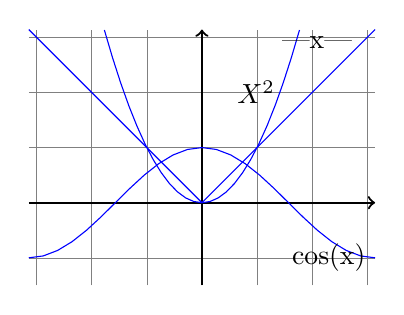
\begin{tikzpicture}[scale = 0.7]
            \draw [help lines] (-pi,-1.5) grid (pi,pi);  %Gitter
            \draw [thick, ->](-pi,0) -- (pi,0);         %x-achse
            \draw [thick, ->](0,-1.5) -- (0,pi);         %y-achse
            \draw [blue, domain=-1.77:1.77] plot (\x, {pow(\x, 2)});
            \node [left] at (1.5,2) {$ X^2$};
            \draw [blue, domain=-pi:pi] plot (\x, {cos(\x r)});
            \node [left] at (pi,-1) {cos(x)};
            \draw [blue, domain=-pi:pi] plot (\x, {abs(\x});
            \node [left] at (2.9,2.9) {|x|};
        \end{tikzpicture}

    \end{minipage}
                
    \begin{minipage}{\linewidth}
        \textbf{Ungerade}\newline
        $f(-t) = -f(t)$ \newline
        Punktsymetrisch am Ursprung
        \[  a_{n} = 0, b_{n} = \frac{4}{T}\int\limits_{0}^{\frac{T}{2}} f(t) \cdot sin(n \omega t)\diff t \]
        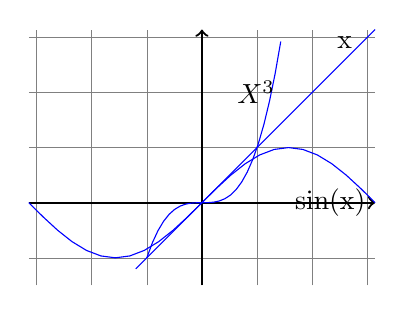
\begin{tikzpicture}[scale = 0.7]
            \draw [help lines] (-pi,-1.5) grid (pi,pi);  %Gitter
            \draw [thick, ->](-pi,0) -- (pi,0);         %x-achse
            \draw [thick, ->](0,-1.5) -- (0,pi);         %y-achse
            \draw [blue, domain=-1:1.43] plot (\x, {pow(\x, 3)});
            \node [left] at (1.5,2) {$ X^3$};
            \draw [blue, domain=-pi:pi] plot (\x, {sin(\x r)});
            \node [left] at (pi,0) {sin(x)};
            \draw [blue, domain= -1.2:pi] plot (\x, {\x});
            \node [left] at (2.9,2.9) {x};
        \end{tikzpicture}

\end{minipage}
\end{multicols}
\clearpage

\section{Lösen von Differentialgleichungen}
\subsection{Allgemeine Vorgehensweisen}
\subsubsection{Trennung von Variablen / Separation}

\begin{tabular}{p{4cm}p{10.5cm}}
\textbf{Form:} $y' = f(x) g(y)$ &
\textbf{Vorgehen:}
\begin{enumerate}
	\item DGL umstellen: $\frac{y'}{g(y)} = f(x)$
	\item Beidseitig nach x integrieren wobei $dx = \frac{dy}{y'}$
	\item Grenzen anpassen: $\int\limits_{y_0=y(x_0)}^{y} \frac{1}{g(y)} dy = \int\limits_{x}^{x_0}f(x) dx$
\end{enumerate}
\end{tabular}
            
\subsubsection{Lineartermsubstitution}

\begin{tabular}{p{5cm}p{10.5cm}}
\textbf{Form:} $y'=f(ax+by+c)$   &
\textbf{Vorgehen:}
\begin{enumerate}
	\item Substitution: $z=ax+by+c$
	\item Einsetzen in $z'=a+bf(z)$
	\item Separation: $\frac{z'}{f(z)} = a + b$ wobei $z_0 = x_0 + y_0$
\end{enumerate}
\end{tabular}
                
\subsubsection{Gleichgradigkeit}
\begin{tabular}{p{4cm}p{10.5cm}}
\textbf{Form:} $y'=f(\frac{y}{x})$ &
\textbf{Vorgehen:}
\begin{enumerate}
	\item Substitution:\quad $z=\frac{y}{x}$
	\item Einsetzen in $z'=\frac{1}{x}(f(z)-z)$
	\item Separation: $\frac{z'}{f(z)-z} = \frac{1}{x}$ wobei $z_0 = \frac{y_0}{x_0}$ 
\end{enumerate}
\end{tabular}
            
\subsection{Differentialgleichung 1. Ordnung}
    
\subsubsection{Konstante Störung $f(x) = A$}
\begin{enumerate}
	\item Homogene Lösung mit $y_h = 0$ berechnen
	
	\item Partikuläre Lösung mit $y_p = B$ (= Konstante) berechnen, indem zeitlich abhängige Terme der DGL ignoriert werden
\end{enumerate}

\subsubsection{Sinusförmige Störung $f(x) = (A \cdot \cos \omega x + B \cdot \sin \omega x)$}
\begin{enumerate}
	\item Homogene Lösung mit $y_h = 0$ berechnen
	
	\item Ansatz für Partikuläre Lösung: $y_p = C \cdot \sin(\omega t) + D\cdot \cos(\omega t)$
	
	\item $y_p$ in DGL einsetzen, $C$ und $D$ per Koeffizientenvergleich ermitteln
\end{enumerate}

\subsection{Störgliedtabelle}
\begin{tabular}{|p{8cm}|p{10cm}|}
    \hline 	
    Störglied $g(x)$ & Ansatz $y_p$ \\
    \hline
    $k$ (Konstante) & $A$ \\
    \hline
    $x^n$ & \multirow{2}{*}{$A_n*x^n + \dots + A_1*x + A_0$} \\
    $p_n(x) = b_n*x^n + \dots + b_1*x + b_0$ & \\
    \hline
    $k*e^{m*x}$ & $A*e^{m*x}$ \\
    \hline	
    $k*cos(b*x)$ & \multirow{3}{*}{$A*cos(b*x) + B*sin(b*x)$} \\
    $k*sin(b*x)$ & \\
    $k_1*cos(b*x) + k_2*sin(b*x)$ & \\
    \hline
    $k*e^{m*x}*cos(b*x)$ & \multirow{3}{*}{$e^{m*x}*(A*cos(b*x) + B*sin(b*x))$} \\
    $k*e^{m*x}*sin(b*x)$ & \\
    $e^{m*x}*(k_1*cos(b*x) + k_2*sin(b*x)$ & \\
    \hline
    $k*cosh(b*x)$ & \multirow{3}{*}{$A*cosh(b*x) + B*sinh(b*x)$} \\
    $k*sinh(b*x)$ & \\
    $k_1*cosh(b*x) + k_2*sinh(b*x)$ & \\
    \hline
    $k*e^{m*x}*cosh(b*x)$ & \multirow{3}{*}{$e^{m*x}*(A*cohs(b*x) + B*sinh(b*x))$} \\
    $k*e^{m*x}*sinh(b*x)$ & \\
    $e^{m*x}*(k_1*cosh(b*x) + k_2*sinh(b*x)$ & \\
    \hline
    $k*x*e^{mx}$ & $(A*x+B)*e^{m*x}$ \\
    \hline
    $p_n(x)*e^{m*x}$ & $(A_n*x^n + \dots + A_1*x + A_0)*e^{mx}$ \\
    \hline
    $x*(k_1*cos(b*x) + k_2*sin(b*x))$ & $(A_1*x+B_1)*cos(b*x) + (A_2*x+B_2)*sin(b*x)$ \\
    \hline
    $x*e^{mx}*(k_1*cos(b*x) + k_2*sin(b*x))$ & $e^{mx}*((A_1*x+B_1)*cos(b*x) + (A_2*x+B_2)*sin(b*x))$ \\
    \hline
    $x*(k_1*cosh(b*x) + k_2*sinh(b*x))$ & $(A_1*x+B_1)*cosh(b*x) + (A_2*x+B_2)*sinh(b*x)$ \\
    \hline
    $x*e^{mx}*(k_1*cosh(b*x) + k_2*sinh(b*x))$ & $e^{mx}*((A_1*x+B_1)*cosh(b*x) + (A_2*x+B_2)*sinh(b*x))$ \\
    \hline
\end{tabular}
\clearpage
\input{idiotenseite/IdiotenseiteInclude}
\pagebreak
%\section{Glossar}
\begin{tabular}{ll}
    GTO & Gate Turn-Off Thyristor \\ 
    IGCT& Integrated Gate-Commutated Thyristor \\ 
    BT  & Bipolarer Transistor  \\ 
    MOS & Metal Oxide Semiconductor \\ 
    IGBT& Insulated-Gate Bipolar Transistor \\ 
\end{tabular} 
\end{document}
